\chapter{Reconstrucción del modelo 3D y textura a partir de una imagen}
\label{Reconstrucción}
En este capítulo se va a detallar como se consigue la reconstrucción 3D del cuerpo humano a partir de una imagen utilizando el método PIFu[\cite{pifu}]. El proceso se puede dividir en varios puntos:

\begin{itemize}
	\item Estudio de los parámetros de test
	\item Generación de la máscara de una imagen
	\item Obtención del modelo 3D
\end{itemize}

\section{Estudio de los parámetros de test}

Lo primero que se tiene que realizar es la instalación del proyecto PIFu[\cite{pifu}] con sus respectivos requerimientos, una vez inicializado, se analizó el proyecto para poder comenzar con la experimentación y obtener modelos. 
De esta manera, se estudió tanto la fase test como la fase de entrenamiento. En este caso solo se ha utilizado la fase de test ya que es la que genera los modelos 3D. Con este estudio se puede observar las necesidades de la red para su correcto funcionamiento, gracias a que se ha podido observar que en realidad la red necesita de 2 imágenes. Una de ellas es la imagen con la cual se busca hacer la representación 3D, y la otra es la máscara de esta imagen. Por otro lado, nos dimos cuenta de que las imágenes han de tener el mismo tamaño y que los tamaños donde mejor trabaja la red es sobre 512x512 píxeles y 1024x1024 píxeles. 
Una vez realizado el estudio se puede comenzar a abarcar los siguientes puntos.

\section{Enmascaramiento de imágenes}

Este proceso nos sirve para quitar información de la imagen inicial, PIFu[\cite{pifu}] por dentro realiza la eliminación del fondo, para ello utiliza la máscara de la imagen. Donde en la imagen dada, los píxeles que tengan el valor de $[255,255,255]$ mantendrá esa información ya que es útil para la red porque es la persona, y los píxeles donde el color sea $[0,0,0]$ será información descartada por la red y se eliminará de la imagen, entendiendo que es el fondo de esta.

En este punto se va a explicar como se ha llegado a obtener la máscara de una imagen.

\subsection{Enmascaramiento de imágenes con el fondo de un sólo color}

Dado que se necesita aparte de la imagen de la persona, la máscara de esta se tuvo que realizar un método que fuese capaz de este proceso, utilizando como base la imagen que se le pasa a la red.

Al inicio se comenzó con imágenes de prueba con fondos blancos o sin fondos, por lo que la extracción es sencilla, todo lo blanco se cambia a negro y el resto de colores diferentes al blanco se cambian al blanco, esto es trivial en python dado que con dos asignaciones obtenemos los resultados que se buscan.
\clearpage
\begin{lstlisting}[caption={Código obtención máscara 1}, label=cod:1]
\end{lstlisting}
\begin{python}
	import numpy as np
	import cv2 
	
	red = [0, 0, 255]
	white = [255, 255, 255]
	black = [0, 0, 0]
	maskpath = 'img_mask.png'
	img = cv2.imread('img.png', cv2.COLOR_RGB2BGR)
	img[np.where((img==red).all(axis=2))] = black
	img[np.where((img!=red).all(axis=2))] = white
	cv2.imwrite(maskpath, img)
\end{python}

El código \ref{cod:1} es capaz de cambiar todo lo rojo a negro y el resto de los colores a blanco.
Con esto se pudo comprobar el funcionamiento de la red utilizando imágenes de prueba.

\subsection{Enmascaramiento de fotos realizadas con teléfonos móviles.}

El punto anterior nos sirvió para comprobar el correcto funcionamiento de la red, pero esto no sirve dado que se busca realizar comparaciones y analizar las métricas de los modelos utilizando el proyecto Tech4diet[\cite{tech}], para ello se hicieron una serie de fotos, donde se usaron dos cámaras diferentes de dos teléfonos móviles diferentes y el uso de una tela verde para facilitar el proceso de enmascaramiento.


\begin{table}[ht]
	\centering
	{\scalefont{0.9}
		\begin{tabular}{@{}lcc@{}}
			\toprule
			Modelo						& 	SM-A528B			&	Mi 9 SE	 	\\ \midrule
			Número Cámaras 				& 	4           		& 	3           	\\
			Cámara Principal			&  64 megapíxeles   	& 48 megapíxeles         	 	\\
			Cámara ultra gran angular 	&  12 megapíxeles		& 13 megapíxeles	\\
			Cámara telefoto		 		&  -					& 8 megapíxeles		\\
			Cámara macro			 	&  5 megapíxeles		& -					\\
			Cámara profundidad		 	&  5 megapíxeles		& -					\\
			Resolución					&  10120x6328 píxeles	& 8000x6000 píxeles		\\
			Apertura focal				&	f/1.8				& f/1.8					\\
			Tamaño del sensor			& 1/1.72" pulgadas		& 1/2" pulgadas			\\ \bottomrule
		\end{tabular}
	}
	\caption{Parámetros de las cámaras elegidas.}
	\label{tablacamara}
\end{table}
\FloatBarrier

Como se puede observar son cámaras con mucha resolución ambas por lo tanto a la hora de hacer las fotos no se encontró ningún problema.

\subsubsection{Preprocesado de las fotos}
Una vez hechas las fotos, estas tuvieron que pasar por un preprocesado antes del enmascaramiento y sucesivamente de usarlas en la red. Para este preprocesado se utilizó la herramienta GIMP[\cite{gimp}]. 
El proceso que se hizo es el siguiente:
\begin{enumerate}
	\item Recorte con la información necesaria.
	\item Escalar imagen.
	\item Creación de un nuevo archivo 1024x1024 con fondo verde y pegar la imagen obtenida después de escalarla.
	\item Retocar colores.
\end{enumerate}
Donde el primer punto se hizo porque como se puede ver en la figura \ref{fig:proceso} en la imagen inicial de la que se parte, la tela verde no ocupa toda la imagen y se busca mantener ese fondo verde.
El segundo punto, es el escalado, pues las imágenes parten de un tamaño de 3468x4624 píxeles, aún habiendo sido recortadas, el tamaño era superior a 1024, por lo que se escala de manera que se cumpla con dicho tamaño.
Una vez hecho esto, se crea un archivo con las medidas necesarias para la red, con el fondo verde y se coloca la imagen después de su escalado.
En ocasiones nos hemos encontrado con errores a la hora del proceso de enmascarado, esto es porque la tela deja pasar la luz y se refleja en el cuerpo, para ello utilizamos un pincel con poca opacidad del color suplementario, en este caso es un color morado, se pinta por encima y con eso se contrarresta la luz verde.

Ya teniendo la imagen como se necesita, se realiza el proceso de generación de máscara, para ello se modificó el código \ref{cod:1}, donde ya no se quiere quitar un color en concreto, si no que en este caso es un rango de color, en este caso se quiere reconocer todos los tipos de verdes posibles.

\begin{lstlisting}[caption={Código obtención máscara 2}, label=cod:2]
\end{lstlisting}
\begin{python}
	import numpy as np
	import cv2 
	
	maskpath = 'img_mask.png'
	img = cv2.imread('img.png')
	hsv = cv2.cvtColor(img, cv2.COLOR_BGR2HSV)
	lower_green = np.array([36, 25, 25])
	upper_green = np.array([70, 255,255])
	mask = cv2.inRange(hsv, lower_green, upper_green)
	result = cv2.bitwise_and(frame, frame, mask=mask)
	b, g, r = cv2.split(result)
	filter = g.copy()
	ret,mask = cv2.threshold(filter,10,255, 1)
	cv2.imwrite(maskpath, maskpath)
\end{python}
\pagebreak

En ambos códigos \ref{cod:1} y \ref{cod:2} se inicializa la imagen y también los colores que se quieren reconocer, y después se realiza el proceso donde se va a generar la máscara, en el código \ref{cod:2} se utiliza el modelo HSV (Hue, Saturation, Brightness - Matiz, Saturación, Brillo) para el rango de color verde.

\section{Obtención del modelo 3D}

La obtención del modelo 3D una vez tenemos la máscara de la imagen es trivial, pues tan solo hay que utilizar la red de PIFu[\cite{pifu}] con la máscara y su imagen respectiva.

\begin{figure}[H]
	\centering
	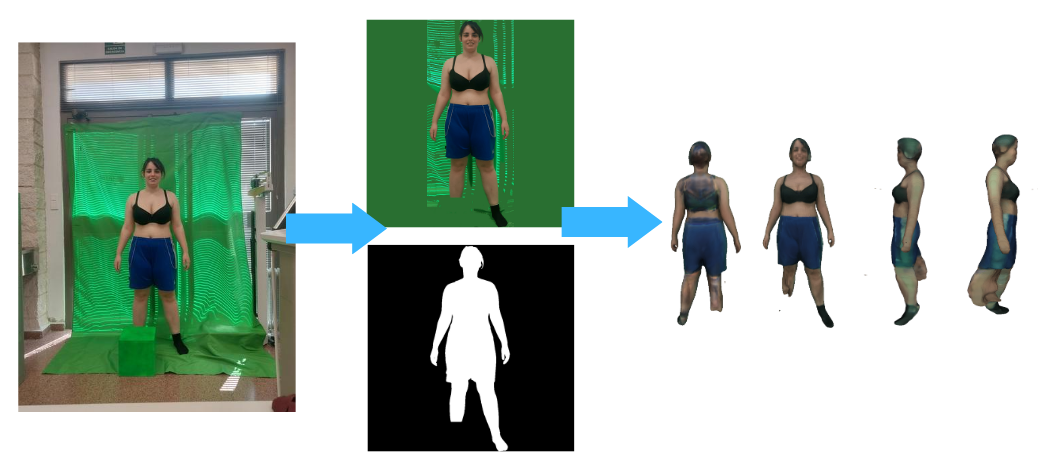
\includegraphics[scale=0.6]{imagenes/proceso1.png}
	\caption{Pipeline usada en para la obtención del modelo. De izquierda a derecha, dada una imagen $I$, se escala, recorta y se ajustan los colores generando la imagen $i$ y se genera la máscara de la imagen $m_i$ a partir de $i$. La red de PIFu[\cite{pifu}] utilizará las imágenes $i$ y $m_i$ para generar el modelo que se ve a la derecha.}
	\label{fig:proceso}
\end{figure}

La figura \ref{fig:proceso} detalla el proceso utilizado. En este proceso se ve como reacciona la red cuando añades ruido en la imagen.

En el apartado \ref{experimentacion} se explica el estudio de los modelos, donde se pueden ver más ejemplos de modelos 3D obtenido por la red.


